\chapter{Test Setups}
\label{chap:\currfilebase}

The test conducted during this thesis isolated features of the prototype system. Measurement data has been compared to a reference system, called MODE3. Both systems are configured to include one impulse hammer, one \ac{DAC} system and one three dimensional accelerometer, as well as a read out computer system with accompanying software.

\section{Hammer-Hammer Test}

The hammer tips of the impact hammers of both the the prototype system and the MODE3 are hit against each other. The targe ot this test is to evaluate the signal quality of the \ac{LC} in the prototype system.

We assume the force transmission from the point of impact to both load cells respectively to be lossless. Thus the recording accuracy of the prototype system is determined by the correlation of the two signal recordings.

The configurations used in the tests are listen in \tabref{tab:hh_config}. The components are shown in \figref{fig:HH_parts}. All hammer-hammer tests were conducted, using a \ac{DAC} of form \figref{fig:dac_comp_simple}

\begin{table}
    \centering
    {\renewcommand{\arraystretch}{1}%
    \footnotesize
    \begin{tabular}{lcc}
        \toprule
        \multicolumn{1}{c}{Sensor Parameter} & \makecell{Reference\\Hammer} & \makecell{Prototype\\Hammer}\\
        \midrule
        Sampling rate & \SI{1600}{\hertz} & \SI{1600}{\hertz}\\
        Dynamic Range & \SIrange{0}{20}{\kilo\newton} & \SIrange{0}{3}{\kilo\newton}\\
        Quantization resolution & \SI{24}{bit} & \SI{12}{bit}\\
        \bottomrule
    \end{tabular}
    \caption[Hammer-Hammer Test Configuration]{Hammer-hammer test configuration}
    \label{tab:hh_config}
    \normalsize
    }
\end{table}

%\\[4ex]
\begin{minipage}{\linewidth}
\centering
\begin{minipage}[b]{0.65\textwidth}
    \centering
    \includestandalone[scale=0.7]{\imgpath/test_setups/HH_parts/HH_parts}
    \captionof{figure}[Hammer-Hammer Test components]{Hammer-Hammer test components}
    \label{fig:HH_parts}
\end{minipage}
\hspace{0em}
\begin{minipage}[b]{0.3\textwidth}
    \centering
    \footnotesize
    \def\circlabel#1#2{%
        \begin{tikzpicture}[%
            x=1em,y=1ex,
            baseline={([yshift=3] N.south)},
            font={\fontsize{6pt}{6.2pt}\selectfont},
            ]%
            \node[%
                circle, fill=white, draw=#1, line width=1pt,
                inner sep=2pt, minimum size=8pt, align=center,
                ] (N) {#2};
        \end{tikzpicture}
    }
    \begin{tabular}{c@{ :\hskip 0.5em}l}
        \toprule
        \large{\circlabel{WesMixL8qual3}{1}} & Piezo + \acs{AMP}\\
        \large{\circlabel{WesMixL8qual3}{2}} & Soft Tip\\
        \large{\circlabel{WesMixL8qual3}{3}} & Tip 34CrMo4\\
        \large{\circlabel{WesMixL8qual3}{4}} & \acs{LC} DYMH-103\\
        \large{\circlabel{WesMixL8qual3}{5}} & \acs{IN-AMP} AD627\\
        \bottomrule
    \end{tabular}
    \normalsize
    \captionof{table}[Legend to Hammer Hammer Test Components]{Legend to \figref{fig:HH_parts}}
    \label{tab:HH_parts}
\end{minipage}
\end{minipage}\\[4ex]

\section{Andromeda Measurement}

In the Andromeda measurement the accelerometers of both systems are positioned at close locations on the Andromeda test bench. Impact hammers of both the prototype and the reference system may be used as input signal. Because of this, the recording of the accelerometer signal of whichever system's impact hammer is not in use, is initiated before the impact and over a longer time frame. To compare signals of both systems, they are synchronized in the post analysis. The target of this test is to evaluate the signal quality of the accelerometer in the prototype system.

The Andromeda test bench consists of a wagon that is supported by a \SI{3}{\meter} long linear drive in the x-axis on two \SI{2.6}{\meter} apart, gantry y-axes that are linear drives as well. Hence kinematic chain
\begin{align*}
    V[b [Y1 Y2] X]
\end{align*}

\figref{fig:andromeda_pics} shows the test setup, while \figref{fig:andromeda_positions} shows an example position of impact in the test setup.

The focus of this test is to compare the accelerometer signals. Therefore, we set the accelerometer parameter as defined in \tabref{tab:set_acc_par}

\begin{table}[!htb]
    \centering
    \def\coltitle#1{\multicolumn{1}{c}{#1}}
    {\renewcommand{\arraystretch}{1.5}%
    \footnotesize
		\begin{tabular}{lccc}
            \toprule
            \makecell{Sensor\\Parameter} &
            \makecell{Sample\\Rate / \si{Hz}} &
            \makecell{Dynamic\\Range / \si{g}} & \makecell{Quanti-\\zation / \si{bit}}\\
            \midrule
            Reference & 1600 & $\pm$5 & 24\\
            Prototype & 1600 & $\pm$4 & 16\\
            \bottomrule
		\end{tabular}
    \normalsize
    }
    \caption[Set Accelerometer Parameters]{Accelerometer parameter settings}
    \label{tab:set_acc_par}
\end{table}

\begin{figure}[!htb]
    \centering
    \subcaptionbox{Andromeda test setup\label{fig:andromeda_pics}}{%
        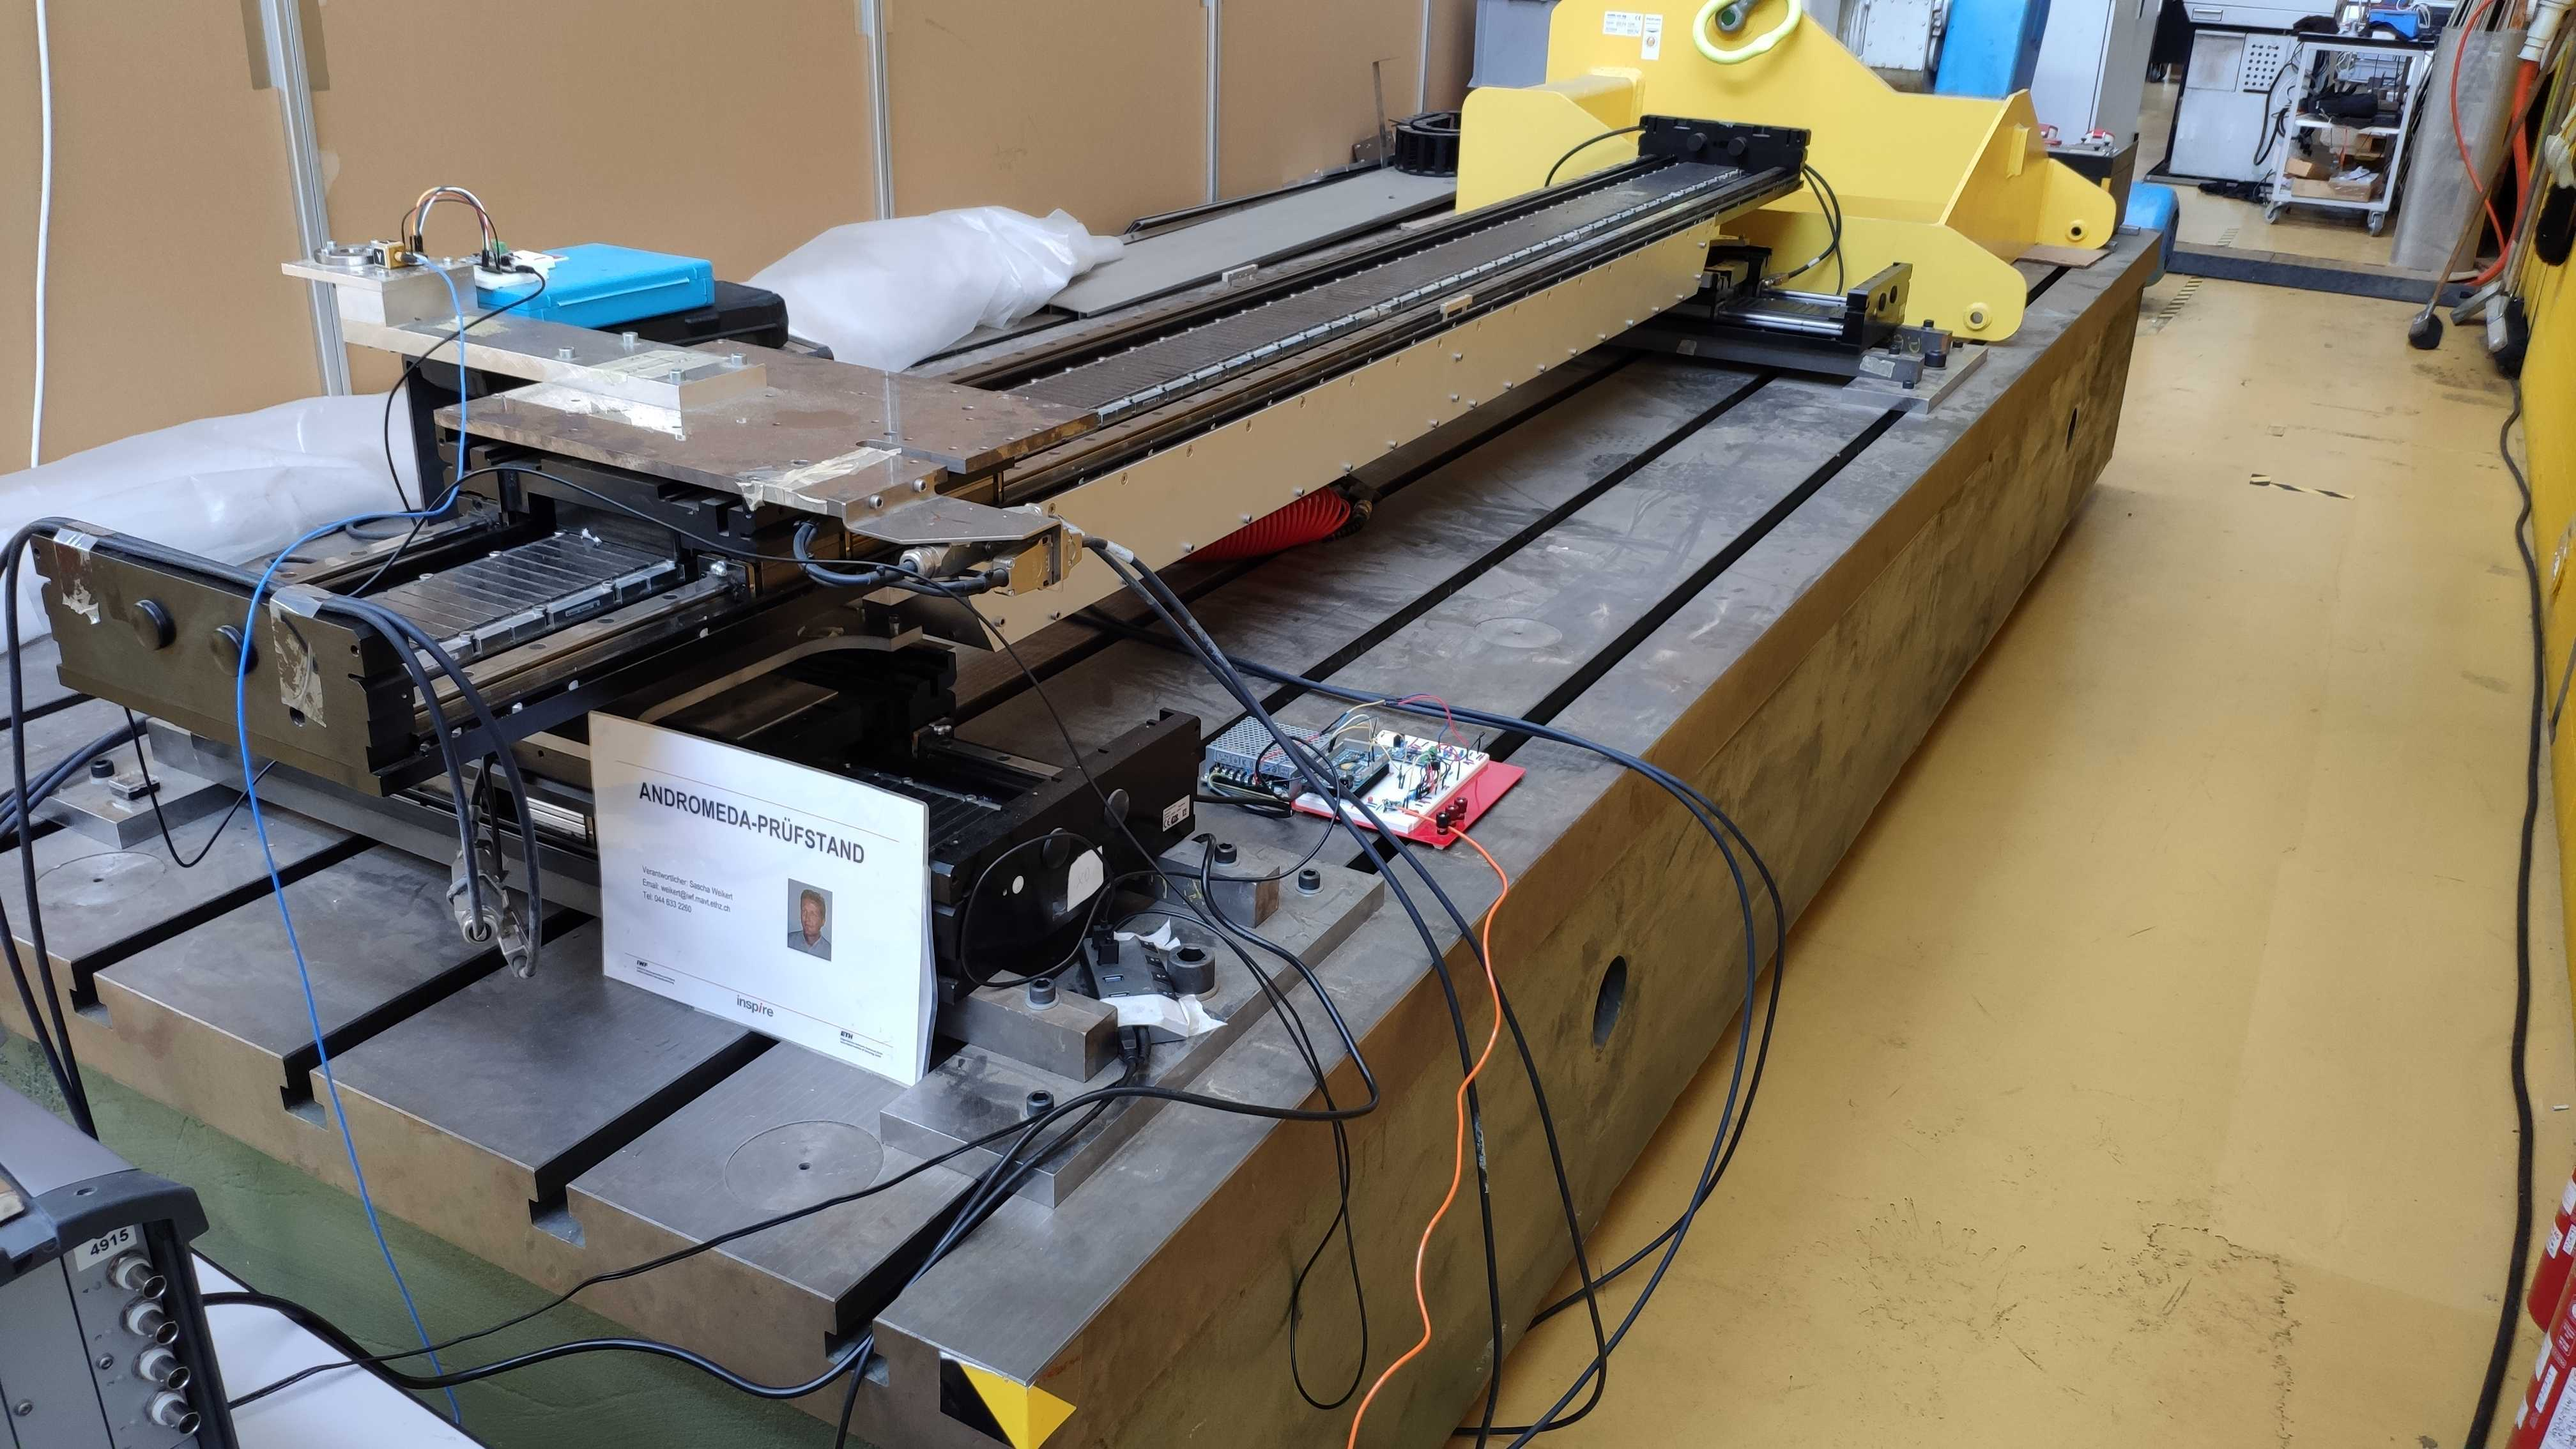
\includegraphics[width=0.55\linewidth]{\imgpath/test_setups/Andromeda/Andromeda_total.jpg}}
        \hspace{4em}
    \subcaptionbox{Acceleromer view\label{sfig:Andromeda_sensors}}{%
        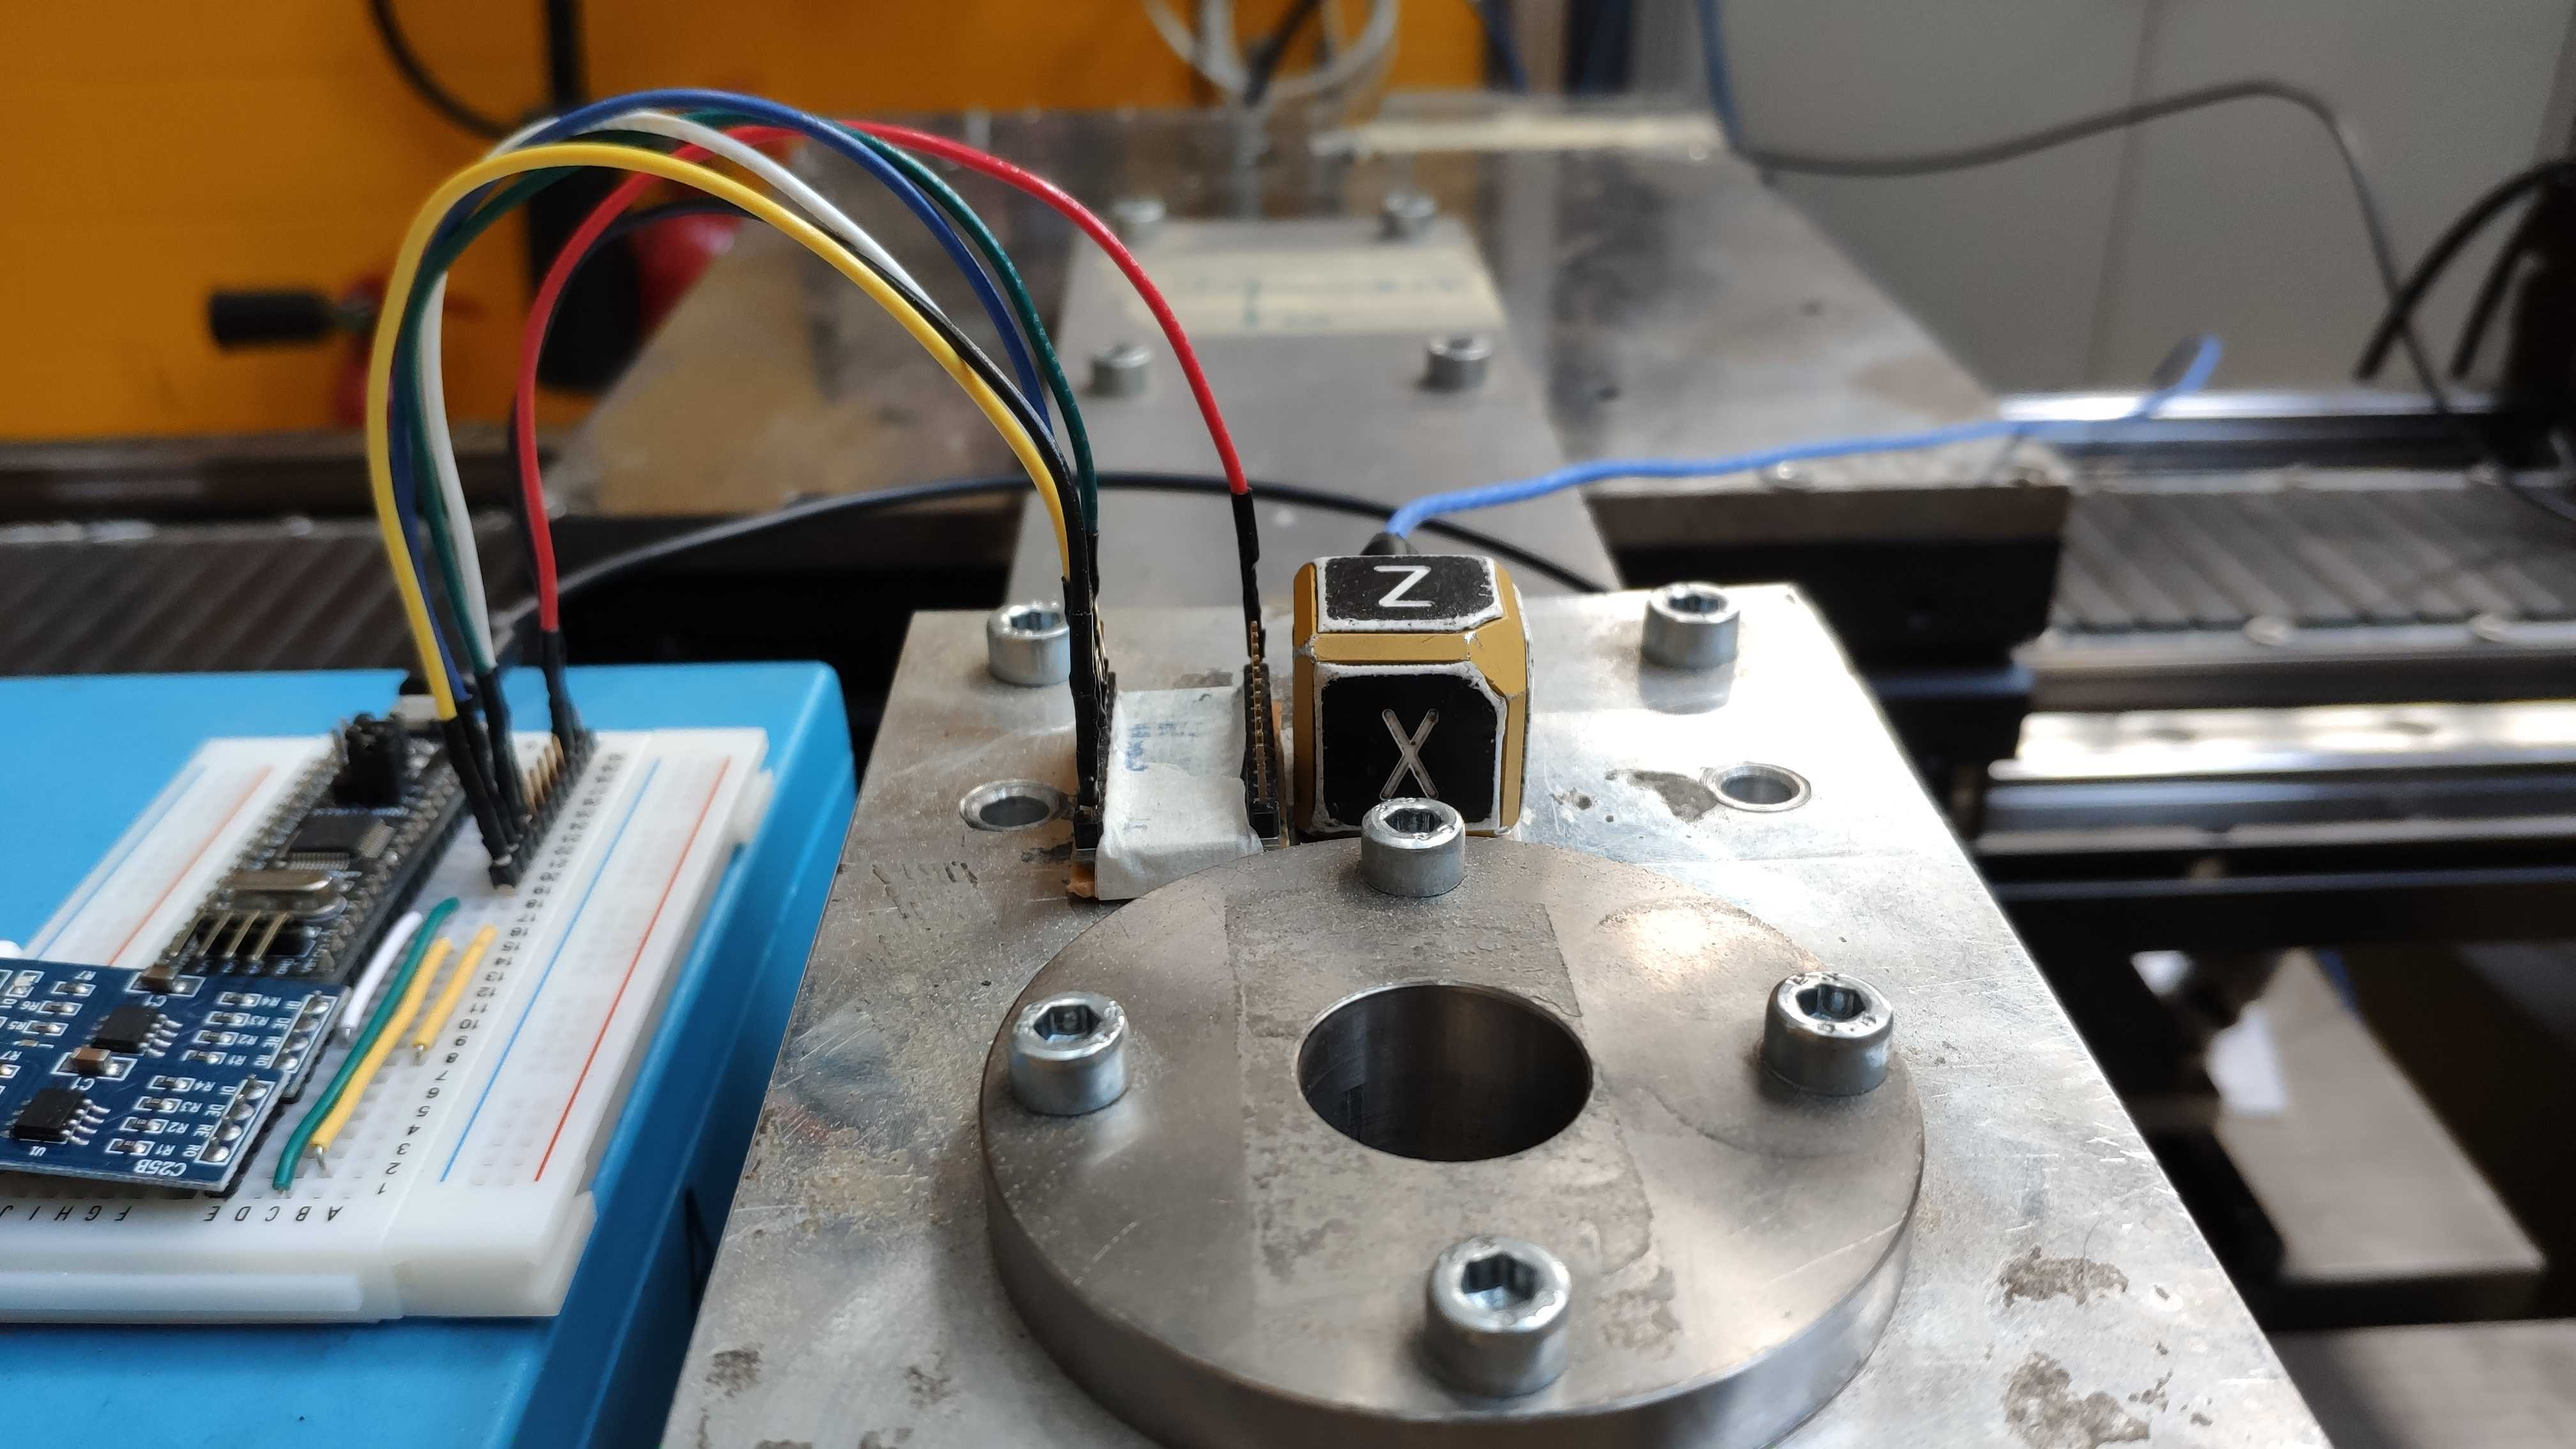
\includegraphics[width=0.3\linewidth]{\imgpath/test_setups/Andromeda/Andromeda_Sensors.jpg}}
    \caption[Andromeda Test Setup]{Andromeda test setup}
    \label{fig:andromeda_pics}
\end{figure}

\begin{figure}[!htb]
    \centering
    \subcaptionbox{Top view\label{sfig:Andromeda_Positions_Top}}{%
        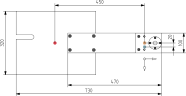
\includegraphics[scale=0.35]{\imgpath/test_setups/Andromeda/Andromeda_Positions_Top}}
        \hspace{4em}
    \subcaptionbox{Trimetric view\label{sfig:Andromeda_Positions_Trimetric_coord}}{%
        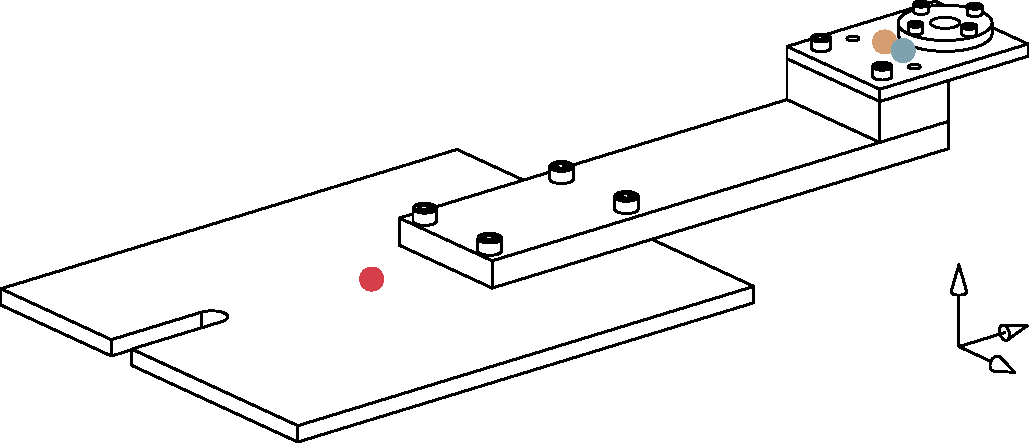
\includegraphics[scale=0.35]{\imgpath/test_setups/Andromeda/Andromeda_Positions_Trimetric_coord}}
    \caption[Andromeda Example Positions]{Andromeda wagon, example impact position}
    \label{fig:andromeda_positions}
\end{figure}

\newpage
\section{Other Test Setups}

To test the bandwidth of the prototype \ac{LC} the hammer tip is hit against a rigid surface. The hardness of the hammer tip determines the bandwidth of the signal. And with hard tips the highest bandwidths can be explored. Apart from the signal measurement tests themselves other tests had to be conducted to guarantee the \ac{DAC} operation and to test the Software. As an example, clock tunable \ac{LPF} are tested in an arduino circuit, that generates a differential sinusoidal signal at different frequencies.


